% SHORT ANSWER QUESTIONS ON INTEGRATION

\ifnum \Version=1
    \part Consider the transform $u=x-1$ and $v=x+y/2$. Then $x = u+1$, and $y = 2v-2u-2$. Using this information, $\displaystyle \int_0^2\int_{4-2x}^{8-2x} \sqrt{x+y/2} \, dy \,dx =  \int_a^b \int_c^d g(u,v) \, dv \, du$,  where $a=\framebox{\strut\hspace{1cm}}$, $b=\framebox{\strut\hspace{1cm}}$, $c=\framebox{\strut\hspace{2cm}}$, $d=\framebox{\strut\hspace{2cm}}$, and the Jacobian of the transform is $J(u,v) = \framebox{\strut\hspace{2cm}}$. 

    \ifnum \Solutions=1 
    {\color{DarkBlue} 
    We need to transform the limits of integration and determine the Jacobian. The Jacobian is
    \begin{align}
        J(u,v) 
        & = \begin{vmatrix} \DXDU & \DXDV \\[8pt] \DYDU & \DYDV \end{vmatrix} 
        = \begin{vmatrix} 1 & 0 \\ -2 & 2 \end{vmatrix} 
        = 2
    \end{align}   
    To work out the limits of integration, we can start by determining the boundaries of the region in the $xy-$plane. The region in the $xy-$plane, $R$, is the set 
    $$R = \{(x,y) \in \mathbb R \, | \, 0 \le x \le 2, \ 4-2x \le y \le 8 - 2x \}$$
    The region in the $xy-$plane is shown below. 
    \begin{center}     
    \begin{tikzpicture}[scale=1.25]
        \begin{axis}[
        axis lines = middle, very thick,
        xlabel = {$x$},
        ylabel = {$y$},
        xmin=-2, xmax=2.95,
        ymin=-2.95, ymax=9.75,
        xtick={0,1,2},
        xticklabels={0,1,2},  
        ytick={0,2,4,6,8},
        yticklabels={0,2,4,6,8}
        ]
        % Plot Top
        \addplot [name path = T,-,domain = 0:2, ultra thick,DarkBlue,samples = 100] {8-2*x} node [right=2pt] {};
        % Plot Bottom        
        \addplot [name path = B,-,domain = 0:2, ultra thick,DarkBlue, samples = 100] {4-2*x} node [very near end, right=4pt] {}; 
        % Plot Left
        \addplot[ultra thick, samples=10, smooth,domain=0:1,DarkBlue] coordinates {(0,4)(0,8)}; 
        % Plot Right
        \addplot[ultra thick, samples=10, smooth,domain=0:1,DarkBlue] coordinates {(2,0)(2,4)};         
        % Labels
        \node[text=DarkBlue] (top) at (1.8,6.5) {$y=8-2x$};
        \node[text=DarkBlue] (top) at (0.7,1) {$y=4-2x$};
        \node[text=DarkBlue] (left) at (-0.65,7) {$x=0$};
        \node[text=DarkBlue] (right) at (2.5,2) {$x=2$};
        \node (l) at (1,4) {$R$};
        % Fill area between paths
        \addplot [black!30, opacity=0.2] fill between [of = T and B, soft clip={domain=0:2}];
        \end{axis}
    \end{tikzpicture}    
    \end{center}     
    To determine the boundaries in the $uv-$plane we transform each of the boundaries individually. 
    \begin{itemize}
        \item \textbf{Left boundary}: using $u = x -1$, the line $x=0$ becomes $u=-1$. 
        \item \textbf{Right boundary}: using $u = x -1$, the line $x=2$ becomes $u=+1$. 
        \item \textbf{Lower boundary}: using $v = x+y/2$, the line $y = 4-2x$ becomes:
        \begin{align}
            y &= 4 - 2x \\
            2x + y & = 4 \\
            x + y/2 &= 2 \\
            v &= 2
        \end{align}
        \item \textbf{Upper boundary}: using $v = x+y/2$, the line $y = 8-2x$ becomes:
        \begin{align}
            y &= 8 - 2x \\
            2x + y & = 8 \\
            x + y/2 &= 4 \\
            v &= 4
        \end{align}
    \end{itemize}
    The region in the $uv-$plane, $G$, is 
    $$G = \{(u,v) \in \mathbb R^2 \, | \, -1 \le u \le 1, \ 2 \le v \le 4 \}$$
    Putting everything together, 
    \begin{align}
        a & = -1 \\
        b &= 1 \\
        c &= 2 \\
        d &= 4 \\
        J &= 2
    \end{align}
    
    \textbf{Additional Notes}\\
    Two additional notes about this question. 
    \begin{itemize}
        \item We were not asked for the integrand $g(u,v)$, but we could work out what it is. First note that 
    \begin{align}
        \sqrt{x+y/2} =  \sqrt v
    \end{align}    
    Thus,
    \begin{align}
        \sqrt{x+y/2} \, dy\,dx = 2\sqrt{v} \,dv \, du \quad \Rightarrow \quad g(u,v) = 2 \sqrt v
    \end{align}
        \item Note that we did not need to obtain $x$ and $y$ in terms of $u,v$, because we were given $x(u,v)$ and $y(u,v)$. But if we needed to express $x$ and $y$ in terms of $u$ and $v$, we could use the expressions for $u$ and $v$ as an augmented matrix and row reduce. 
    \begin{align}
        \begin{pmatrix} 1 & 0 & u+1 \\1 & 1/2 & v\end{pmatrix} 
        \sim \begin{pmatrix} 1 & 0 & u+1 \\0 & 1 & 2v-2u-2\end{pmatrix} 
    \end{align}
    Thus
    \begin{align}
        x &= u+1 \\
        y &= 2v-2u-2
    \end{align}
    
    \end{itemize}
    
    
    }
   \else

   \fi
\fi 

\ifnum \Version=2
% SPHERICAL EXERCISE
% VERBATUM FROM SPRING 2022 QUIZ
% hand written solution only
\part $\displaystyle I = \int_{-3}^3 \int_{-\sqrt{9-x^2}}^{\sqrt{9-x^2}} \int_0^{\sqrt{9-x^2-y^2}}z\sqrt{x^2+y^2+z^2} \, dz\, dy \, dx = \int_a^b\int_0^d\int_0^k f(\rho,\phi,\theta) \, d\rho \, d\phi \, d\theta$, where $a = \framebox{\strut\hspace{1cm}}$, $b = \framebox{\strut\hspace{1cm}}$, $d = \framebox{\strut\hspace{1cm}}$, $k = \framebox{\strut\hspace{1cm}}$, $f(\rho,\phi,\theta) = \framebox{\strut\hspace{2cm}}$. 

\ifnum \Solutions=1 {\color{DarkBlue} \textit{Solutions:} a screen capture from a hand-written solution from a previous offer of MATH 2551 is below. 
    \begin{figure}[h]
    \centering
    \includegraphics[width=14cm]{202302/FinalExam/Images/ImgFE.FITB.3.01.png}
    \end{figure}  
    
    } 
   \else
      
   \fi
    
\fi


% POLAR
% Ready
% 15.6
% FINE FOR EXAM
\ifnum \Version=3
    \part $R$ is the region in the first quadrant bounded by the lines $x=0$, $y=0$, and the curve $x^2+y^2=9$. Then $R$ has area $M$, and using polar coordinates for integration, the $y-$coordinate of the centroid of $R$ is $\bar y = M_x/M$, where $M_x = \int_a^b \int_c^d f(r,\theta) \, dr \, d\theta$,  and $a=\framebox{\strut\hspace{1.0cm}}$, $b=\framebox{\strut\hspace{1.0cm}}$, $c=\framebox{\strut\hspace{1cm}}$, $d=\framebox{\strut\hspace{1cm}}$, and $f(r,\theta) = \framebox{\strut\hspace{2cm}}$. 
    
    \ifnum \Solutions=1 
    {\color{DarkBlue}
    The region is bounded by 
    $$0\le r \le 3, \quad 0\le \theta \le \pi/2$$
    Thus
    \begin{align}
        \bar y &= \frac1M \int_{0}^{\pi/2}\int_{0}^{2} (r\sin\theta) r \, dr \, d\theta
    \end{align} 
    Thus,
    \begin{align}
        a &= 0 \\
        b &= \pi/2 \\
        c&= 0 \\
        d&= 3 \\
        f(r,\theta) &= r^2\sin\theta
    \end{align}
    }
   \else

   \fi
    
\fi




% READY
\ifnum \Version=4
    \part $\displaystyle \int_{0}^{1}\int_{0}^{z} \int_0^{z-y} \, dx \, dy \, dz = \int_a^b \int_c^d \int_h^k \, dz \, dy\,dx$, where $a=\framebox{\strut\hspace{0.8cm}}$, $b=\framebox{\strut\hspace{0.8cm}}$, $c=\framebox{\strut\hspace{1.0cm}}$, $d=\framebox{\strut\hspace{1.0cm}}$, $h=\framebox{\strut\hspace{1.6cm}}$, $k=\framebox{\strut\hspace{1.6cm}}$.
    
    \ifnum \Solutions=1 
    {\color{DarkBlue} \textit{Solutions:}
    Note the following
    \begin{itemize}
        \item From the given integral, all variables are non-negative, so the solid lives in the first octant.
        \item Also from the given integral, we know $z$ is at most 1.
        \item The innermost bounds for the $x$ integral gives us that $x \le z - y$, or $z \ge x+y$. So the solid lives above the plane z = x+y, and below the plane $z = 1$. In other words, $$x+y \le z \le 1$$ This gives us the limits for $z$ in the new integral. 
        \item To get the $y$ bounds in the new integral, project the solid down onto the $xy$-plane. The top of the solid has the edge $z = 1 = x+y$, and projecting the top edge down onto the xy-plane gives you $1=x+y$, or $y = 1-x$.
    \end{itemize}
    Putting these ideas together we obtain:
    $$\displaystyle \int_{0}^{1}\int_{0}^{z} \int_0^{z-y} \, dx \, dy \, dz = \int_0^1 \int_0^{1-x} \int_{x+y}^1  \, dz \, dy \,dx$$
    It wasn't necessary to integrate, but if we did we would find that the volume is $1/6$. 
    }
    \else

    \fi
    
\fi


% 
\ifnum \Version=5

    \part $\displaystyle \int_{0}^{1}\int_{\sqrt x}^{1} \int_0^{1-y} \, dz \, dy \, dx = \int_a^b \int_c^d \int_0^k \, dx \, dz\,dy$, where $a=\framebox{\strut\hspace{0.8cm}}$,  $b=\framebox{\strut\hspace{0.8cm}}$, $c=\framebox{\strut\hspace{1.4cm}}$, $d=\framebox{\strut\hspace{1.4cm}}$, $k=\framebox{\strut\hspace{1.4cm}}$.

    % stewart 13.7 # 31

    \ifnum \Solutions=1 
    {\color{DarkBlue} \textit{Solutions:}
    $$\displaystyle \int_{0}^{1}\int_{\sqrt x}^{1} \int_0^{1-y} f(x,y,z) \, dz \, dy \, dx = \int_0^1 \int_0^{1-y} \int_0^{y^2} f(x,y,z) \, dx \, dz \,dy$$
    So
    \begin{align}
        a &= 0 \\
        b &= 1 \\
        c &= 0 \\
        d &= 1-y \\
        k &= y^2
    \end{align}
    }
    \else

    \fi
    
\fi


% READY CAN BE USED ANYWHERE, MAYBE A SAMPLE EXAM? 
\ifnum \Version=6
% SHORT SPHERICAL AND CYLINDRICAL EXERCISE
% VERBATUM FROM SPRING 2022 QUIZ
% hand written solution only
\part Point $P$ has rectangular (Cartesian) coordinates $(x,y,z) = (0,-3,4)$ in $\mathbb R^3$. In cylindrical coordinates, the point is $(r,\theta,z)$, and in spherical coordinates the point is $(\rho, \phi, \theta)$. Where $r=\framebox{\strut\hspace{1cm}}$, $\theta=\framebox{\strut\hspace{1cm}}$, $z=\framebox{\strut\hspace{1cm}}$, $\rho=\framebox{\strut\hspace{1.5cm}}$, and $\phi=\framebox{\strut\hspace{3cm}}$.

\ifnum \Solutions=1 {\color{DarkBlue} \textit{Solutions:} In cylindrical: 
 $$\displaystyle (r,\theta,z) = (3,\frac{3\pi}2,4)$$
 In spherical 
 $$\displaystyle (\rho, \phi, \theta) = \left(5,\arctan\left(\frac34\right),\frac{3\pi}2 \right)$$
 A screen capture from a hand-written solution from a previous offer of MATH 2551 is below. 
    \begin{figure}[h]
    \centering
    \includegraphics[width=14cm]{202302/FinalExam/Images/ImgFE.FITB.3.02.png}
    \end{figure}  
    \newpage
    } 
   \else
      
   \fi
    
\fi





% SIDEWAYS PARABOLA AND A LINEAR
% READY FOR 2024
\ifnum \Version=7
    \part The area of the region bounded by $x=-y^2$ and $x+y+2=0$ is $\displaystyle  \int_a^b \int_c^d f(x,y) \, dx \, dy$,  where $a=\framebox{\strut\hspace{1cm}}$, $b=\framebox{\strut\hspace{1cm}}$, $c=\framebox{\strut\hspace{2cm}}$, $d=\framebox{\strut\hspace{2cm}}$, and $f(x,y) = \framebox{\strut\hspace{2cm}}$.
    
    \ifnum \Solutions=1 
    {\color{DarkBlue} We want to determine where the two curves intersect. Setting them equal to each other: 
    \begin{align}
        -y^2 &= -y-2 \\
        0 &= y^2 - y - 2 \\
        0 &= (y-2)(y+1) \\
        y &= 2, -1
    \end{align}
    To obtain the $x-$coordinates, we can use either curve. Substituting the two $y-$values into either curve gives us intersection points at $(-4,2)$ and at $(-1,-1)$. It can help to sketch the two curves, as shown in the diagram below. 
       \begin{center}     
    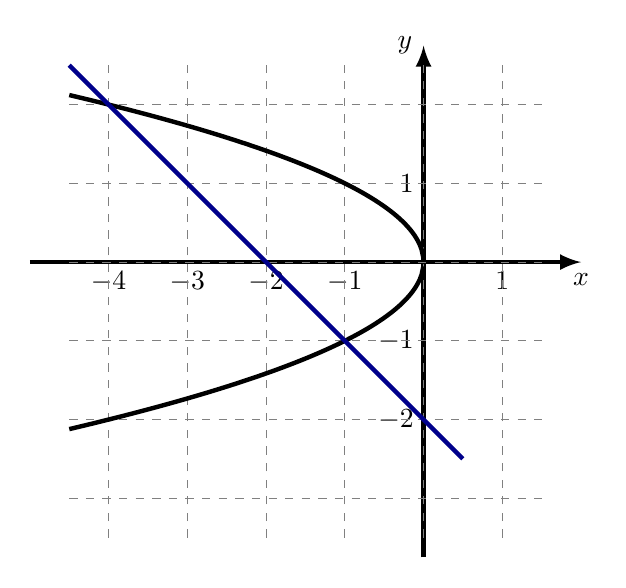
\begin{tikzpicture}[scale=1.0]
      \draw[ultra thick,->,>=latex] (-5,0)--(2,0) node[below] {$x$};
      \draw[ultra thick,->,>=latex] (0,-3.75)--(0,2.75) node[left] {$y$};
      \draw (-1,0) node[below] {$-1$};          
      \draw (-2,0) node[below] {$-2$};          
      \draw (-3,0) node[below] {$-3$};          
      \draw (-4,0) node[below] {$-4$};          
      \draw (1,0) node[below] {$1$};
      \draw (0,1) node[left] {$1$};        
      \draw (0,-1) node[left] {$-1$};
      \draw (0,-2) node[left] {$-2$};
      \draw[help lines,gray,thin,dashed] (-4.5, -3.5) grid (1.5, 2.5);
      \draw[domain=-4.5:0,ultra thick,samples=200] plot ({\x},{sqrt(-\x )});
      \draw[domain=-4.5:0,ultra thick,samples=200] plot ({\x},{-sqrt(-\x )});
      \draw[domain=-4.5:0.5,ultra thick,DarkBlue,samples=200] plot ({\x},{-\x-2});
    \end{tikzpicture}
    \end{center}     
    The region is bounded on the \textbf{right} by $x=-y^2$, and bounded on the \textbf{left} by $x=-y-2$. The region is 
    $$R = \{(x,y) \in \mathbb R^2 \, | \, -1\le y \le 2, \quad -y-2 < x < -y^2\}$$
    Therefore, 
    \begin{align}
        a & = -1 \\
        b &= +2 \\
        c &= -y -2 \\
        d &= -y^2 \\
        f &= 1
    \end{align}
    }
   \else

   \fi
\fi 


% TETRAHEDRON IN FIRST QUADRANT
\ifnum \Version=8

    \part The volume of the tetrahedron cut from the first octant by the plane $8x+2y+z=24$ is $\displaystyle \int_A^B \int_0^D \int_0^K   \, dz\, dy \,dx$, where $A=\framebox{\strut\hspace{1.2cm}}$, $B=\framebox{\strut\hspace{1.2cm}}$, $D=\framebox{\strut\hspace{3cm}}$, and $K=\framebox{\strut\hspace{3cm}}$.
    
    \ifnum \Solutions=1 
    {\color{DarkBlue} \textit{Solutions:}
    We consider each of the variables individually, starting with the outermost integral and working our way to the innermost integral. 
    \begin{itemize}
        \item \textbf{Outermost integral}: When $y=z=0$, the plane cuts the $x$-axis at the point where $$8x + 0 + 0 = 24$$ Or where $x=3$. So every point in the solid has $x$-coordinates between $x=0$ and $x=3$. 
        \item \textbf{Middle integral}: When $z=0$, the plane cuts the $xz$-plane along the line 
        \begin{align}
            8x+2y + 0 &= 24 \\
            y &= 12-4x
        \end{align}
        So every point in the solid has $y$-coordinates between $y=0$ and $y=12-4x$. 
        \item \textbf{Innermost Integral}: for any given $x$ and $y$ in the solid, points in the solid will have a $z-$coordinate between $0$ and $z=24-8x-2y$. 
        \begin{align}
            0 \le y \le 24-8x-2y
        \end{align}
    \end{itemize}

    The triple integral is
    $$\displaystyle \int_{0}^{3}\int_{0}^{12-4x} \int_0^{24-8x-2y} \, dz \, dy \, dx$$
    Therefore,
    \begin{align}
        A &= 0 \\
        B &= 3 \\
        D & = 12-4x\\
        K &= 24-8x-2y
    \end{align}
    }
    \else

    \fi
    
\fi



% 15.6
% CENTROID Y-COORDINATE PARABOLA AND LINE
\ifnum \Version=9
    \part A thin plate with density $4x$ is bounded in the $xy-$plane by $y=4-x^2$ and $y=2-x$. The plate has mass $M$. The $y-$coordinate of the centroid is $\bar y = M_x/M$, where $\displaystyle M_x = \int_A^B \int_C^D f(x,y) \, dy \, dx$,  and $A=\framebox{\strut\hspace{1cm}}$, $B=\framebox{\strut\hspace{1cm}}$, $C=\framebox{\strut\hspace{3cm}}$, $D=\framebox{\strut\hspace{3cm}}$, and $f(x,y) = \framebox{\strut\hspace{3cm}}$. 
    
    \ifnum \Solutions=1 
    {\color{DarkBlue}
    The region is bounded by 
    $$2-x \le y \le 4-x^2$$
    The given curves intersect when 
    \begin{align}
        2-x &= 4-x^2\\
        0 &= x^2-x-2 \\
        &= (x-2)(x+1)
    \end{align}
    The curves intersect at $x=-1,2$. Using $y=2-x$, the intersection points are $(-1,3)$ and $(2,0)$. The region is shown below. 
    \begin{center}  
        \begin{tikzpicture}[scale=1.25]
            \begin{axis}[
            axis lines = middle, very thick,
            xlabel = {$x$},
            ylabel = {$y$},
            xmin=-5, xmax=5.75,
            ymin=-2.5, ymax=5.75,
            xtick={-4,-2,0,2,4},
            xticklabels={-4,-2,0,2,4},
            ytick={-2,0,2,4},
            yticklabels={-2,0,2,4}        
            ]
            % Curves
            \addplot [name path = A,-,domain = -2.2:2.5, line width=0.8mm,DarkBlue,samples = 30] {4-x^2} ;
            \addplot [name path = C,-,domain = -2.2:3, line width=0.8mm,DarkBlue,samples = 4] {2-x} ;
            % Fill area between paths
            \addplot [black!30, opacity=0.2] fill between [of = A and C, soft clip={domain=-1:2}];
            \end{axis}
        \end{tikzpicture}    
    \end{center}   
        
    Thus
    \begin{align}
        \bar y &= \frac{M_x}M = \frac1M \int_{-1}^{2}\int_{2-x}^{4-x^2} 4xy \, dy \, dx
    \end{align} 
    Thus
    \begin{align}
        A &= -1 \\
        B &= 2 \\
        C&= 2-x \\
        D&= 4-x^2 \\
        f(x,y) &= \delta y = 4xy
    \end{align}
    We shouldn't leave the answer in terms of $\delta$ unless $\delta$ is defined somewhere in the student answers, because we need to know what $\delta$ is equal to. 
    }
   \else

   \fi
    
\fi




% 15.2
% TRIANGULAR REGION, TWO INTEGRALS TO ONE
\ifnum \Version=10
    \part $\displaystyle \int_{-3}^{1} \int_{-x}^{3} f(x,y) d y \, d x + \int_{1}^{5} \int_{x-2}^{3} f(x,y) d y \, d x = \int_{a}^{b} \int_{c}^{d} f(x,y) \, d x\,  d y$, where 
    $a=\framebox{\strut\hspace{1.4cm}}$, $b=\framebox{\strut\hspace{1.4cm}}$, $c=\framebox{\strut\hspace{3cm}}$, and $d=\framebox{\strut\hspace{3cm}}$.    

    \ifnum \Solutions=1 
    {\color{DarkBlue}
    We are given two regions: 
    \begin{align}
        R_1: &\ -3 \le x \le 1, \quad -x \le y \le 3 \\
        R_2: &\ 1 \le x \le 5, \quad x-2 \le y \le 3
    \end{align}
    It can help to sketch the region, as shown in the diagram below. 
       \begin{center}     
        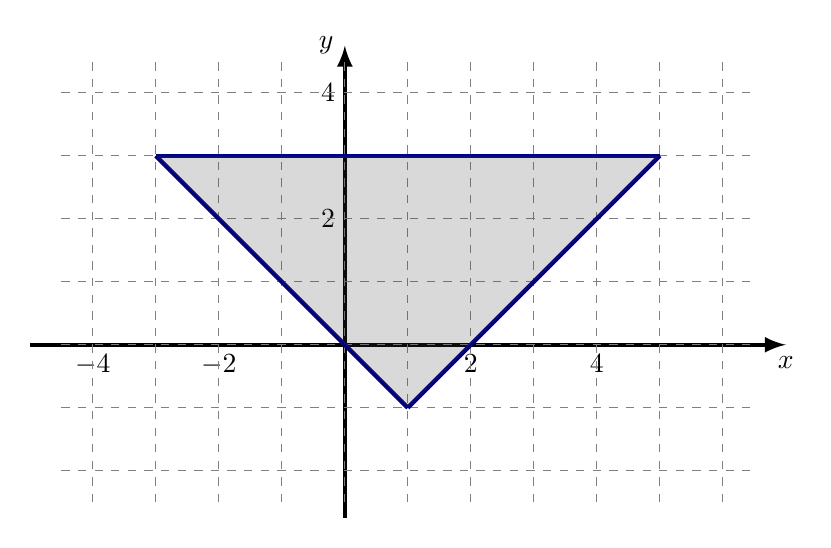
\begin{tikzpicture}[scale=0.8]
        \draw[ultra thick,->,>=latex] (-5,0)--(7,0) node[below] {$x$};
        \draw[ultra thick,->,>=latex] (0,-2.75)--(0,4.75) node[left] {$y$};
        \draw (-4,0) node[below] {$-4$};          
        \draw (-2,0) node[below] {$-2$};          
        \draw (2,0) node[below] {$2$};          
        \draw (4,0) node[below] {$4$};          
        \draw (0,2) node[left] {$2$};        
        \draw (0,4) node[left] {$4$};
        \draw[help lines,gray,thin,dashed] (-4.5, -2.5) grid (6.5, 4.5);
        \draw[domain=-3:1,ultra thick,DarkBlue,samples=4] plot ({\x},{-\x });
        \draw[domain=1:5,ultra thick,DarkBlue,samples=4] plot ({\x},{\x-2});
        \draw[ultra thick,-,DarkBlue,>=latex] (-3,3)--(5,3);
        \draw[fill=gray!50!black, opacity=0.2] (-3,3) -- (1,-1) -- (5,3);                
    \end{tikzpicture}
    \end{center}      
    The region is also
    \begin{align}
            -y \le x \le y+2, \quad -1 \le y \le 3
    \end{align}
    Thus
    \begin{align}
        V = \int_{-1}^3\int_{-y}^{y+2} f(x,y) \, dx\, dy
    \end{align}
    }
   \else
   \fi
\fi 




\ifnum \Version=11

    \part $\displaystyle \int_{-1}^1 \int_{x^2}^1 \int_0^{1-y} dz \, dy \, dx = \int_a^b \int_c^d \int_h^k  \, dx \, dz \,dy$, where 
    $a=\framebox{\strut\hspace{1.0cm}}$, $b=\framebox{\strut\hspace{1.0cm}}$, $c=\framebox{\strut\hspace{1.4cm}}$, $d=\framebox{\strut\hspace{1.4cm}}$, $h=\framebox{\strut\hspace{2.0cm}}$,
    $k=\framebox{\strut\hspace{2.0cm}}$.

    \ifnum \Solutions=1 
    {\color{DarkBlue} We are given
    \begin{align}
        -1 \le \, &x \le 1 \\
        x^2 \le \, &y \le 1 \\
        0 \le \, &z \le 1-y 
    \end{align}
    Thus,
    \begin{align}
        0 \le \, &y \le 1 \\
        0 \le \, &z \le 1-y \\
        -\sqrt{y} \le \, &x \le \sqrt{y}
    \end{align}
    The triple integral becomes
    \begin{align}
        \int_{-1}^1 \int_{x^2}^1 \int_0^{1-y} dz \, dy \, dx 
        = \int_a^b \int_c^d \int_h^k  \, dx \, dz \,dy 
        = \int_0^1 \int_0^{1-y} \int_{-\sqrt y}^{\sqrt y}  \, dx \, dz \,dy 
    \end{align}
    Thus,
    \begin{align}
        a &= 0 \\
        b &= 1 \\
        c &= 0 \\
        d &= 1-y \\
        h &= -\sqrt y\\
        k &= \sqrt y
    \end{align}
    }
   \else

   \fi
    
\fi


\ifnum \Version=12
    \part Consider the transform $u=x+y$ and $v=x-y$. Then $x = (u+v)/2$, and $y = (u-v)/2$, and $\displaystyle \int_0^2\int_{y-2}^{2-y}  \, dx \,dy =  \int_a^b \int_c^d g(u,v) \, dv \, du$,  where $a=\framebox{\strut\hspace{2cm}}$, $b=\framebox{\strut\hspace{2cm}}$, $c=\framebox{\strut\hspace{2cm}}$, $d=\framebox{\strut\hspace{2cm}}$, and the Jacobian of the transform is $J(u,v) = \framebox{\strut\hspace{2cm}}$. 

    \ifnum \Solutions=1 
    {\color{DarkBlue} 
    We need to transform the limits of integration. The region in the $xy-$plane, $R$, is the set 
    $$R = \{(x,y) \in \mathbb R \ | \ 0 \le y \le 2, \ y-2 \le x \le 2-y \}$$
    The triangular region is shown below. 
    \begin{center}     
    \begin{tikzpicture}[scale=1]
        \begin{axis}[
        axis lines = middle, very thick,
        xlabel = {$x$},
        ylabel = {$y$},
        xmin=-2.5, xmax=2.5,
        ymin=-0.8, ymax=3.2,
        xtick={-2,-1,0,1,2},
        xticklabels={-2,-1,0,1,2},  
        ytick={0,1,2,3},
        yticklabels={0,1,2},
        ymajorgrids=true,
        xmajorgrids=true,
        grid style=dashed    
        ]
        % Plot Right
        \addplot [name path = R, -, domain = -2:0, line width=0.8mm,DarkBlue, samples = 100] {2+x} node [right=2pt] {};
        % Plot Left
        \addplot [name path = L, -, domain = 0:2, line width=0.8mm,DarkBlue, samples = 100] {2-x} node [right=2pt] {};
        \node (l) at (0.6,0.55) {$R$};
        \addplot [name path = T,-, domain = -2:2, line width=0.8mm,DarkBlue,samples = 100] {0} node [very near end, right=4pt] {}; 
        % Fill area between paths
        \addplot [black!30, opacity=0.2] fill between [of = R and T, soft clip={domain=-2:0}];
        \addplot [black!30, opacity=0.2] fill between [of = L and T, soft clip={domain=0:+2}];
        \end{axis}
    \end{tikzpicture}    
    \end{center}     
    
    To determine the boundaries in the $uv-$plane we transform each of the boundaries individually. 
    \begin{itemize}
        \item \textbf{Right boundary}: using $u=x+y$, the line $x=2-y$ becomes $u=2$. 
        \item \textbf{Left boundary}: using $v=x-y$, the line $x=y-2$ becomes $v=-2$. 
        \item \textbf{Bottom boundary}: using $y=(u-v)/2$, the line $y=0$ becomes $u=v$.
    \end{itemize}
    It isn't necessary to sketch the region in the $uv-$plane, but it can help when determining the limits of integration in the transformed integral. The region is shown below. 
    \begin{center}     
    \begin{tikzpicture}[scale=1]
        \begin{axis}[
        axis lines = middle, very thick,
        xlabel = {$u$},
        ylabel = {$v$},
        xmin=-2.75, xmax=2.75,
        ymin=-2.75, ymax=2.75,
        xtick={-3,-2,-1,0,1,2,3},
        xticklabels={-3,-2,-1,0,1,2,3},  
        ytick={-2,-1,0,1,2},
        yticklabels={-2,-1,0,1,2},
        ymajorgrids=true,
        xmajorgrids=true,
        grid style=dashed      
        ]
        \node (l) at (.85,-1) {$G$};
                % Plot 1
        \addplot [name path = T, -,domain = -2:2, ultra thick,DarkBlue, samples = 4] {x} node [right=2pt] {};
        \addplot[name path = R, ultra thick, samples=4, smooth,domain=0:1,DarkBlue] coordinates {(2,-2)(2,2)};    
        \addplot[name path = B, ultra thick, samples=4, smooth,domain=0:1,DarkBlue] coordinates {(-2,-2)(2,-2)};    
        % Fill area between paths
        \addplot [black!30, opacity=0.2] fill between [of = B and T, soft clip={domain=-2:2}];
        \end{axis}
    \end{tikzpicture}    
    \end{center}         
    The region in the $uv-$plane, $G$, is 
    $$G = \{(u,v) \in \mathbb R^2 \, | \, -2 \le u \le 2, \ -2 \le v \le u \}$$
    
    \textbf{Jacobian and $g(u,v)$ }\\
    The Jacobian is
    \begin{align}
        J(u,v) 
        & = \begin{vmatrix} \DXDU & \DXDV \\[8pt] \DYDU & \DYDV \end{vmatrix} 
        = \begin{vmatrix} 1/2 & 1/2 \\ 1/2 & -1/2 \end{vmatrix} 
        = -1/4 - 1/4 = - 1/2
    \end{align}      
    The function $g(u,v)$ is $|J| = 1/2$.    
    \vspace{12pt}
    
    \textbf{Putting Everything Together}\\
    Therefore, 
    \begin{align}
        a & = -2 \\
        b &= 2 \\
        c &= -2 \\
        d &= u \\
        J &= -1/2
    \end{align}

    }
   \else

   \fi
\fi 


% READY
% GOOD BUT NOT NEEDED? 
\ifnum \Version=13
    \part $\displaystyle \int_1^{e}\int_{\ln(x)}^{1} \, dy \, dx = \int_a^b \int_c^d dx \, dy$ where $a=\framebox{\strut\hspace{0.8cm}}$, $b=\framebox{\strut\hspace{0.8cm}}$, $c=\framebox{\strut\hspace{0.8cm}}$, $d=\framebox{\strut\hspace{0.8cm}}$.
\ifnum \Solutions=1 
    After changing the order of integration $\displaystyle 
        \int_1^{e}\int_{\ln(x)}^{1} f(x,y) \, dy \, dx
        {\color{DarkBlue} \ = \int_0^{1}\int_{1}^{e^y} f(x,y) dx dy }$.
   \else

   \fi
\fi 




\ifnum \Version=14
    \part A change of variables of the form $u=x+y, \ v = x - y$, defines a transform from the $xy-$plane to the $uv-$plane. The Jacobian of the transform from the $uv$-plane to the $xy-$plane is $J(u,v) = \partial (x,y)/\partial (u,v) = \framebox{\strut\hspace{1.5cm}}$, where $x(u,v) = \framebox{\strut\hspace{1.5cm}}$ and $y(u,v) = \framebox{\strut\hspace{1.5cm}}$.
    \ifnum \Solutions=1 \\[12pt]
    {\color{DarkBlue} In the context of the given coordinate transformation, we consider a transformation from a set of coordinates $(u, v)$ to the set of coordinates $(x, y)$. The Jacobian matrix for this transformation is defined as

    $$ \displaystyle  J = \begin{pmatrix} \frac{\partial x}{\partial u} & \frac{\partial x}{\partial v} \\ \frac{\partial y}{\partial u} & \frac{\partial y}{\partial v} \end{pmatrix} $$
    
    We do not have $x$ and $y$ in terms of $u$ and $v$. Solving for $x$ and $y$ using an augmented matrix,
    \begin{align}
        \begin{pmatrix} 1 & 1 & u \\1 & -1 & v\end{pmatrix} 
        \sim \begin{pmatrix} 1 & 1 & u \\0 & -2 & v - u\end{pmatrix} 
        \sim \begin{pmatrix} 1 & 1 & u \\0 & 1 & u/2-v/2\end{pmatrix} 
        \sim \begin{pmatrix} 1 & 0 & u/2+v/2 \\0 & 1 & u/2-v/2\end{pmatrix} 
    \end{align}
    Thus
    \begin{align}
        x &= u/2+v/2\\
        y &= u/2-v/2
    \end{align}
    And
    \begin{align}
        J(u,v) & = \begin{vmatrix} \DXDU & \DXDV \\[8pt] \DYDU & \DYDV \end{vmatrix} = \begin{vmatrix} \frac12 & \frac12 \\ \frac12 & -\frac12 \end{vmatrix} = -\frac14-\frac14 = - 1/2
    \end{align}
    Note that the Jacobian of a transform can be negative. When using the Jacobian in an integral we use the absolute value of the Jacobian. 
    }
   \else

   \fi
\fi 


% READY
% SHOULD USE AS A PRACTICE BECAUSE IT IS ONLY ONE PART?
\ifnum \Version=20
% SHORT JACOBIAN
\part Consider the coordinate transformation $x=3v-u$, $y = 2u+v$. The Jacobian $J(u,v) = \frac{\partial (x,y)}{\partial(u,v) }$ is $J = \framebox{\strut\hspace{1cm}}$.

\ifnum \Solutions=1 {\color{DarkBlue} We are given
    \begin{align}
        x &= 3v-u\\
        y &= 2u+v
    \end{align}
    And
    \begin{align}
        J(u,v) & = \begin{vmatrix} \DXDU & \DXDV \\[8pt] \DYDU & \DYDV \end{vmatrix} = \begin{vmatrix} -1 & 3 \\ 2 & 1 \end{vmatrix} = -7
    \end{align}
    The Jacobian of a transform can be negative.     
    } 
   \else
   \fi
\fi


